\documentclass[tocnopagenum]{thesis-ekf}
%a4paper, 12pt, 1.5-es sortávolság, margók
\usepackage[T1]{fontenc}
\PassOptionsToPackage{defaults=hu-min}{magyar.ldf}
\usepackage[magyar]{babel}
\usepackage{mathtools,amssymb,amsthm,pdfpages}
\footnotestyle{rule=fourth}
\usepackage{comment}
\usepackage{enumitem}

\newtheorem{tetel}{Tétel}[chapter]
\theoremstyle{definition}
\newtheorem{definicio}[tetel]{Definíció}
\theoremstyle{remark}
\newtheorem{megjegyzes}[tetel]{Megjegyzés}

\begin{document}
	\institute{Matematikai és Informatikai Intézet}
	\title{Informatikai eszközökkel támogatott sport és egészségfejlesztés}
	\author{Sipos Levente\\Szak: Programtervező informatikus BSc\\Specializáció: Szoftverfejlesztő informatikus}
	\supervisor{Dr. Király Roland\\beosztás}
	\city{Eger}
	\date{2022}
	\maketitle
	\tableofcontents

	\addcontentsline{toc}{chapter}{Bevezetés}
	\addcontentsline{toc}{chapter}{Összegzés}
	\chapter*{Bevezetés}
	\begin{comment}
		Ezek később lesznek hasznosak
		\begin{tetel}
			Tétel szövege.
		\end{tetel}
		
		\begin{proof}
			Bizonyítás szövege.
		\end{proof}
		
		\begin{definicio}
			Definíció szövege.
		\end{definicio}
		
		\begin{megjegyzes}
			Megjegyzés szövege.
		\end{megjegyzes}
	\end{comment}
	\chapter*{Összegzés}


	
	\verb*|#TODO|: Összefoglalás...
	\bibliographystyle{plain}
	\bibliography{references}
	
	% Aláírt, szkennelt nyilatkozat beillesztése a szakdolgozat végére
	%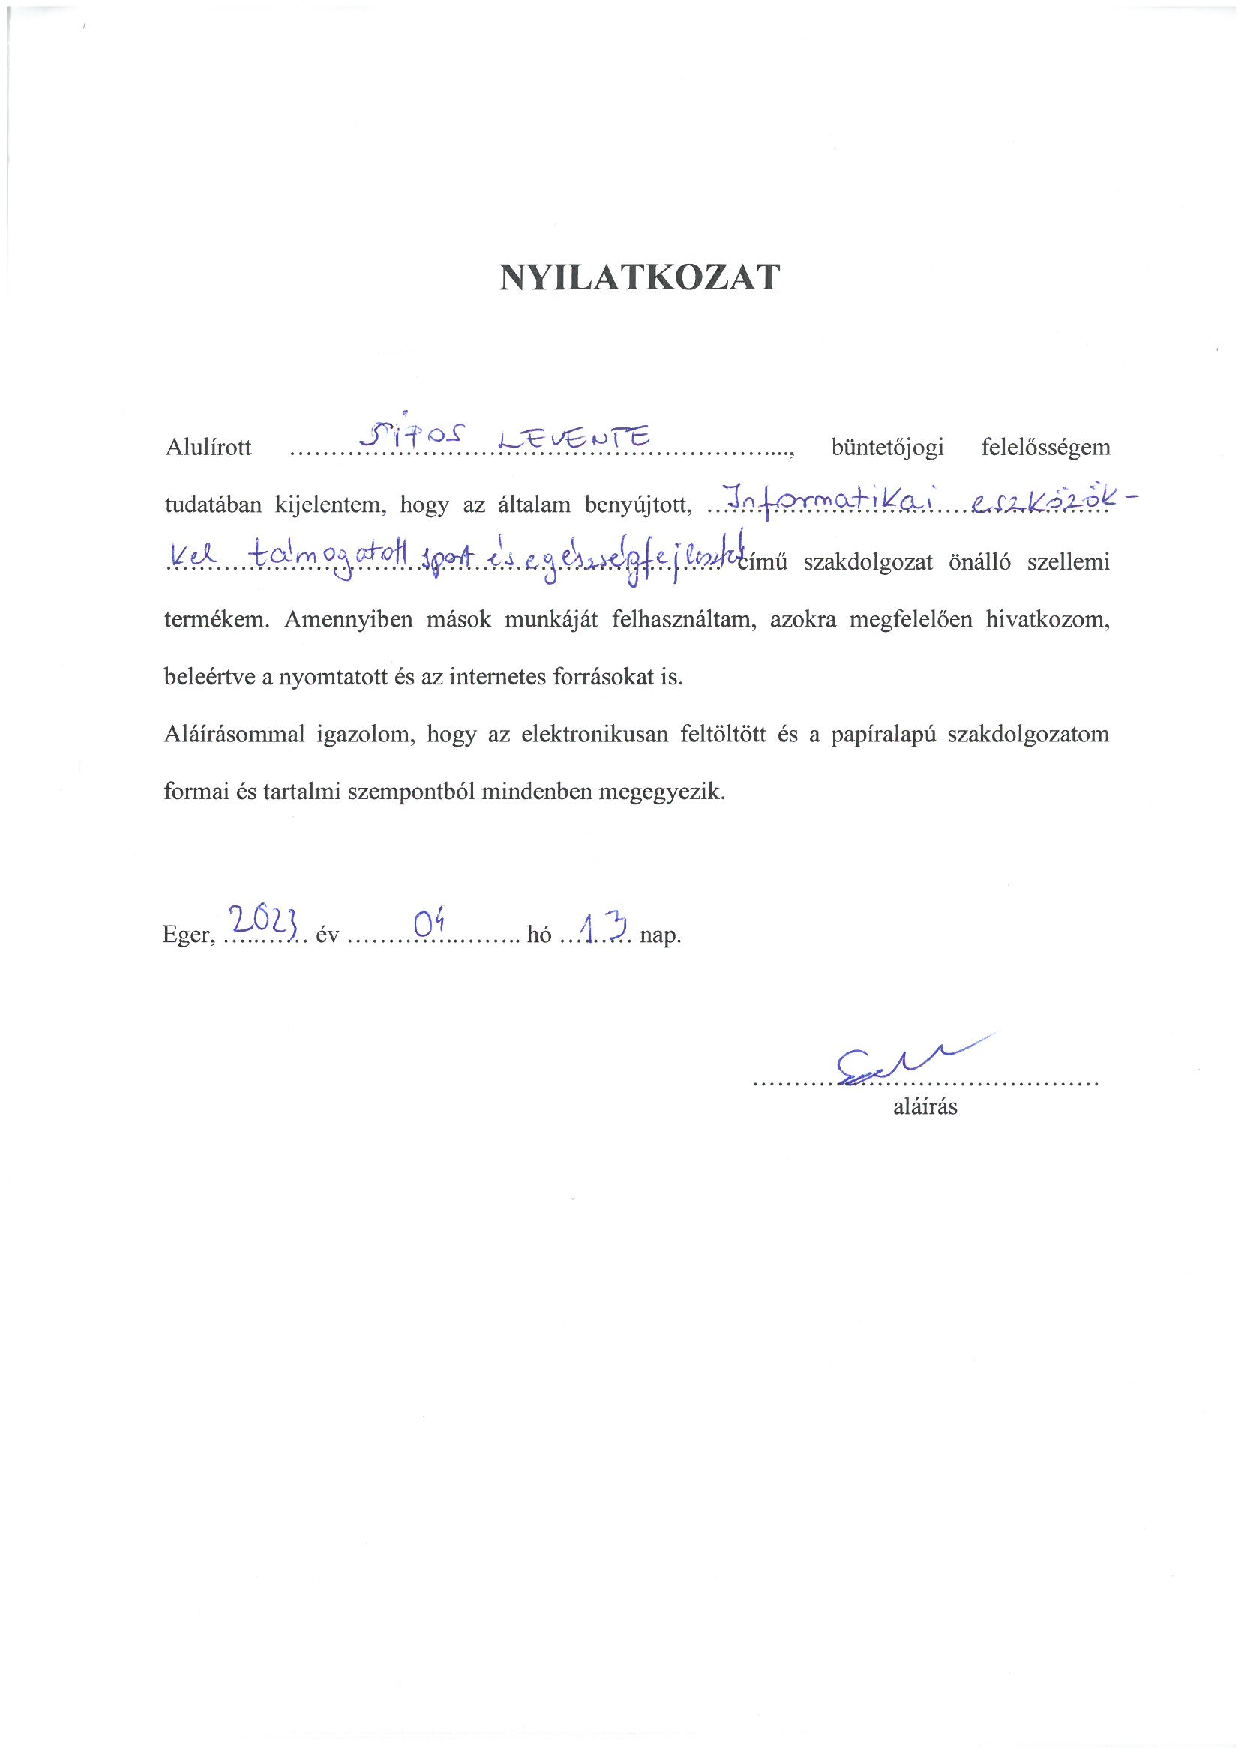
\includepdf{nyilatkozat.pdf}
\end{document}